% !TEX root = ../featureselection.tex

\section{Case Study}
Throughout our paper, we have used a running example of a team
of clinical researchers using predictive modeling to
classify patients at high risk of developing diabetes.
In this section, we describe how \infuse has led to a variety
of insights when exploring the features of the models.

\begin{figure*}[ht]
\centering
\resizebox{0.9\linewidth}{!}{%
\begin{tikzpicture}
\newcommand*{\imgwidth}{3.7cm}
\newcommand*{\boxsize}{0.437cm}
\newcommand*{\boxpos}{(.295, -.18)}
\newcommand*{\rightimagepos}{(4.8, 0)}
\newcommand*{\leftimagepos}{(0, 0)}
\node[inner sep=0pt] at \leftimagepos
    {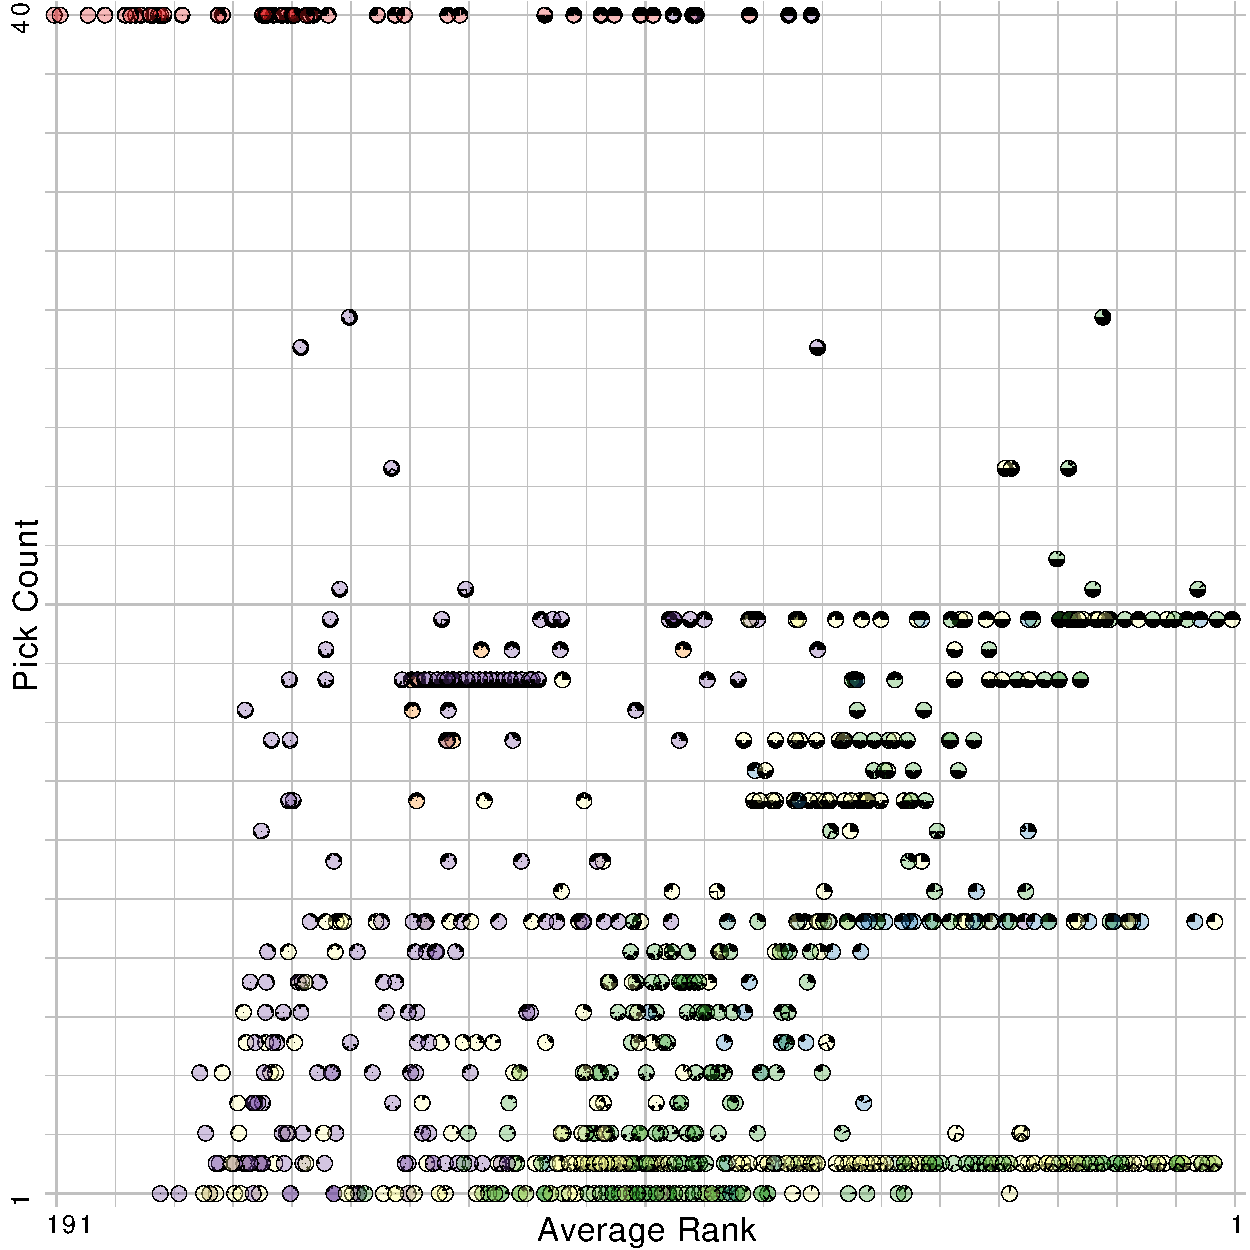
\includegraphics[width=\imgwidth]{infuse/ap}};
\node[inner sep=0pt] at \leftimagepos
    {\phantom{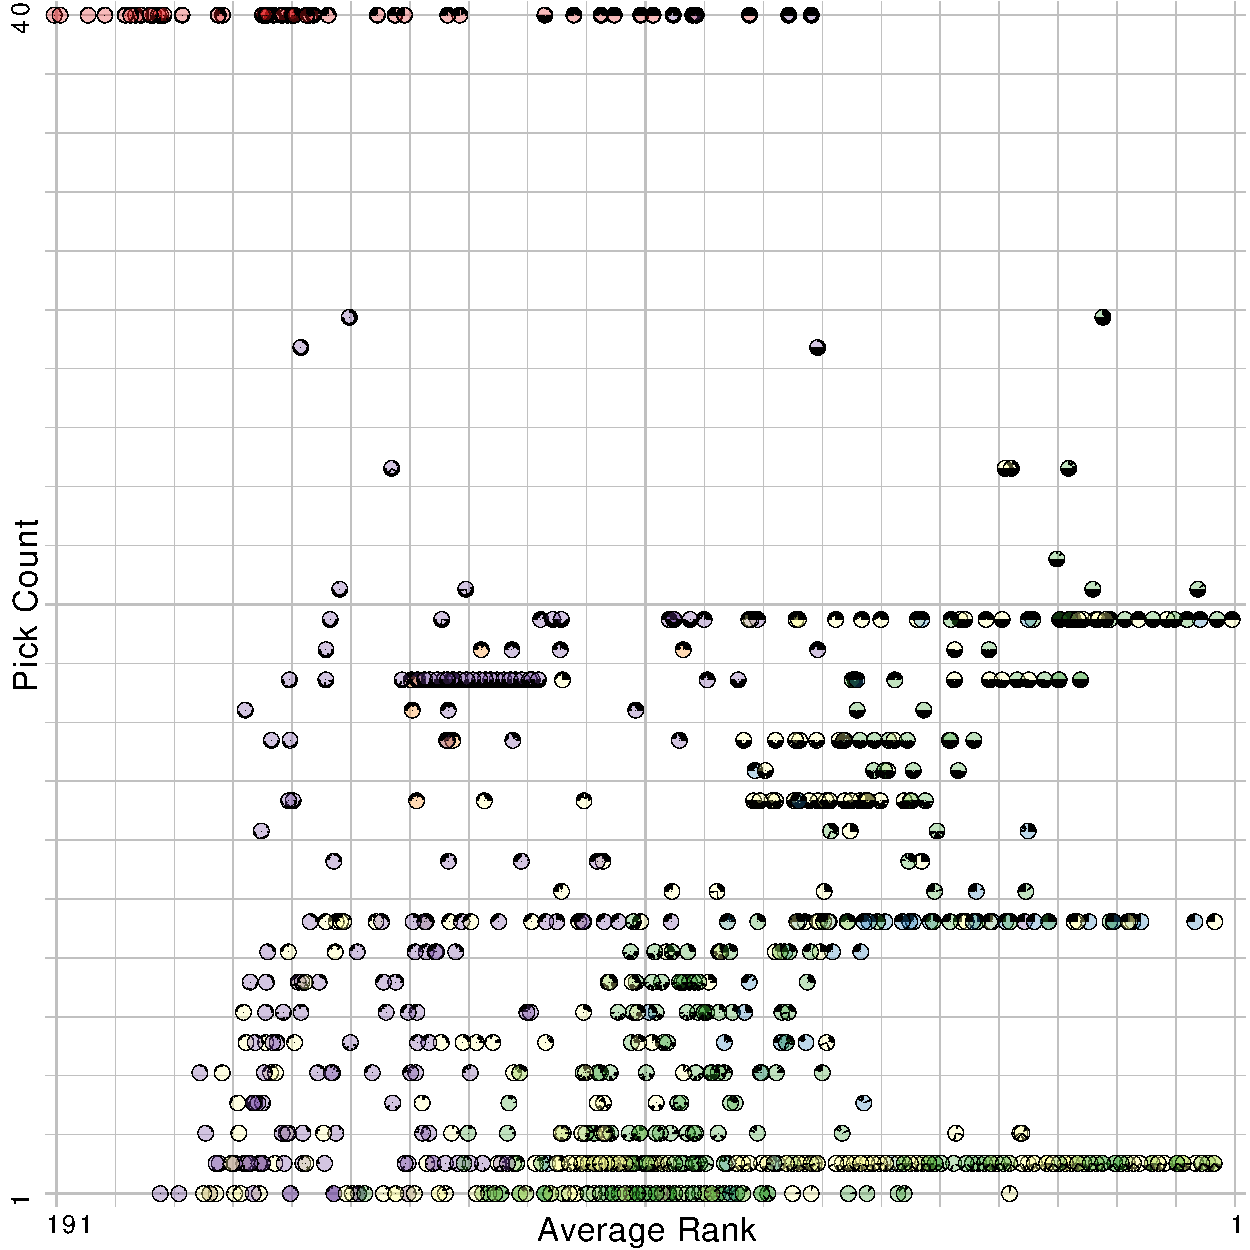
\includegraphics[width=\imgwidth]{infuse/ap}}};
\node[inner sep=2.5pt,very thick, text height=\boxsize] (zoom)
at \boxpos
    {\hspace*{\boxsize}};
\node[inner sep=-0.05pt] (lasso) at \rightimagepos
    {\phantom{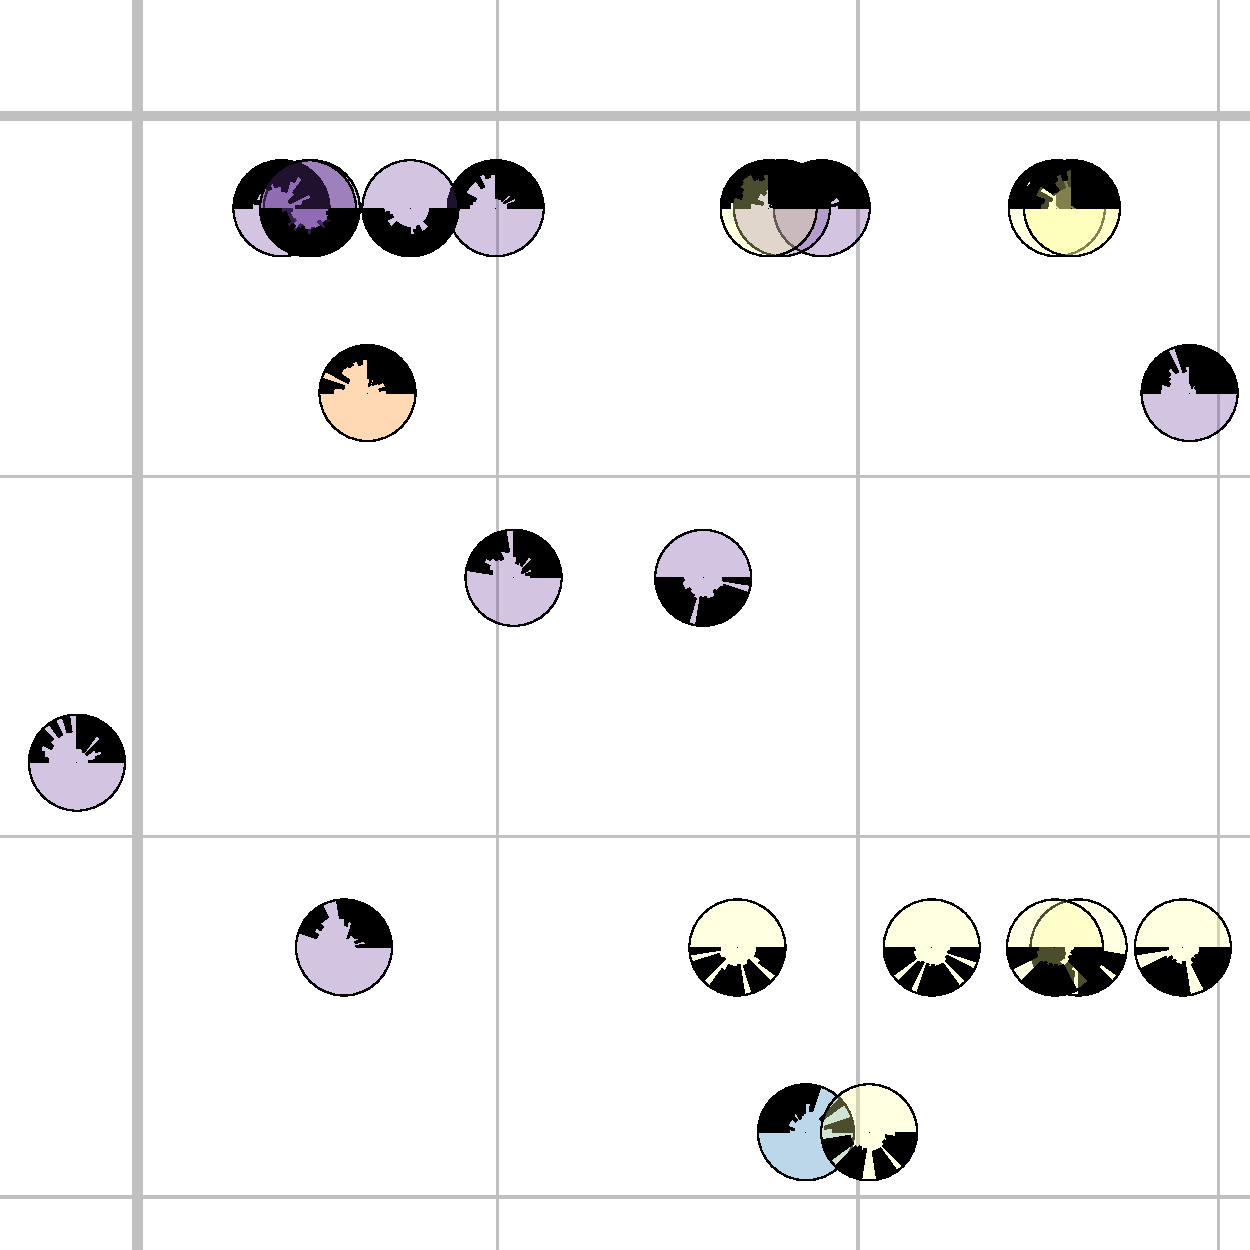
\includegraphics[width=\imgwidth]{infuse/lasso}}};
\draw (zoom.north west) -- (lasso.north west);
\draw (zoom.south west) -- (lasso.south west);
\draw (zoom.north east) -- (lasso.north east);
\draw (zoom.south east) -- (lasso.south east);
\node[very thick, draw=red!90, text height=\boxsize]
at \boxpos {\hspace*{\boxsize}};
\node[inner sep=0pt, very thick] at \rightimagepos
    {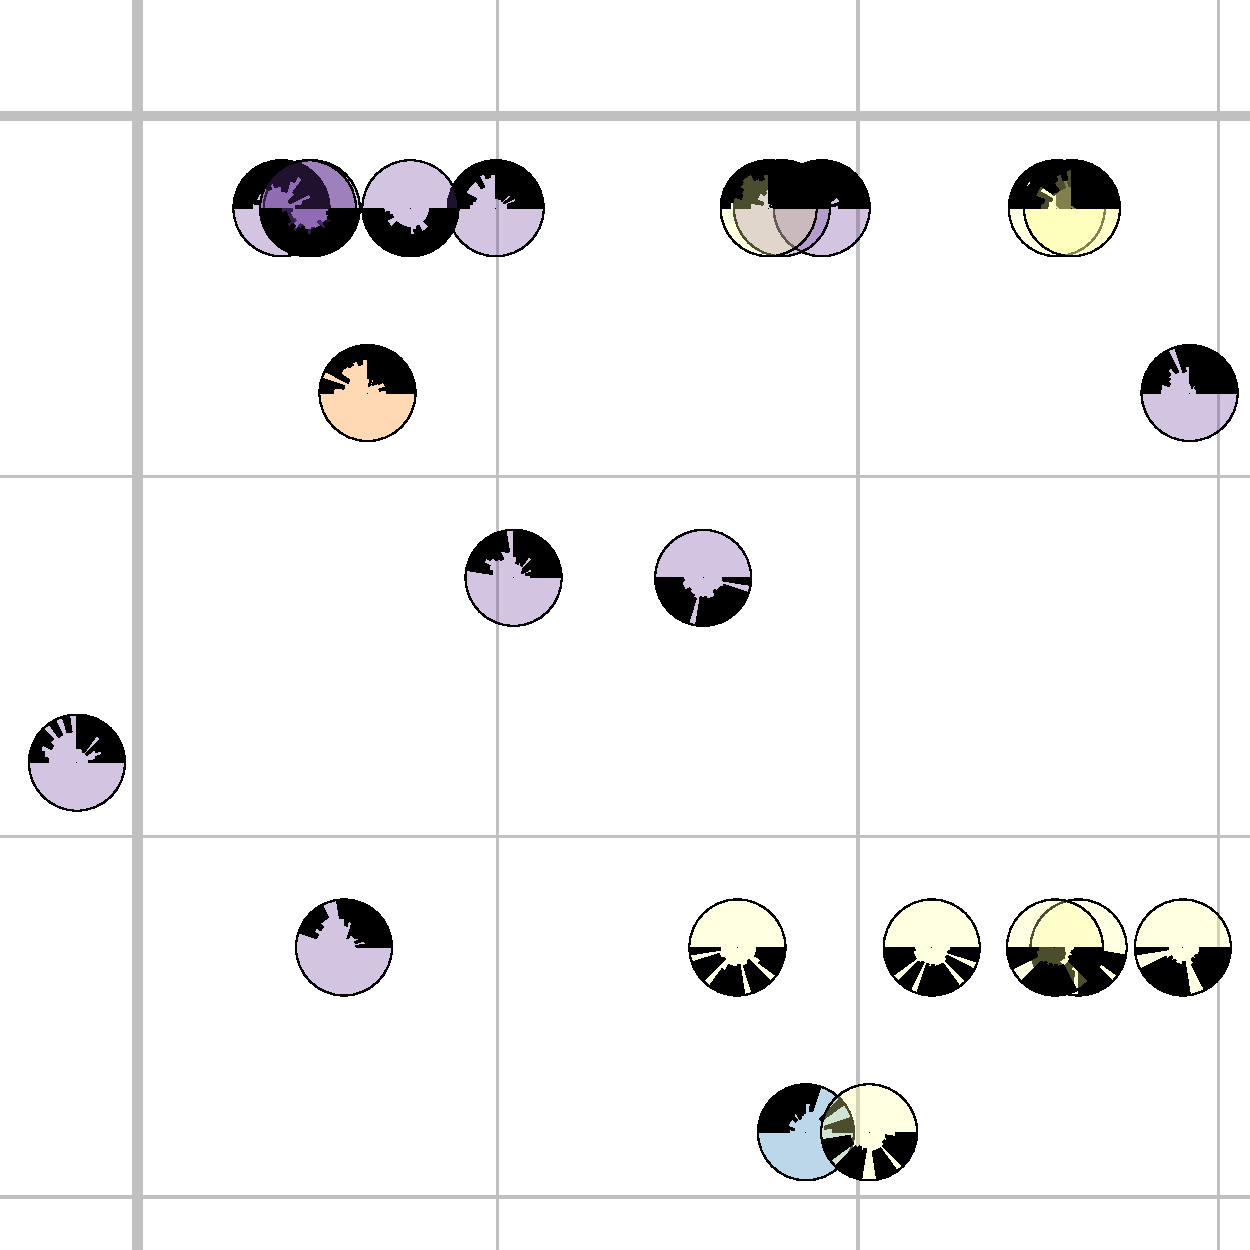
\includegraphics[width=\imgwidth]{infuse/lasso}};
\node[inner sep=0pt, very thick, draw=red!90] at \rightimagepos
    {\phantom{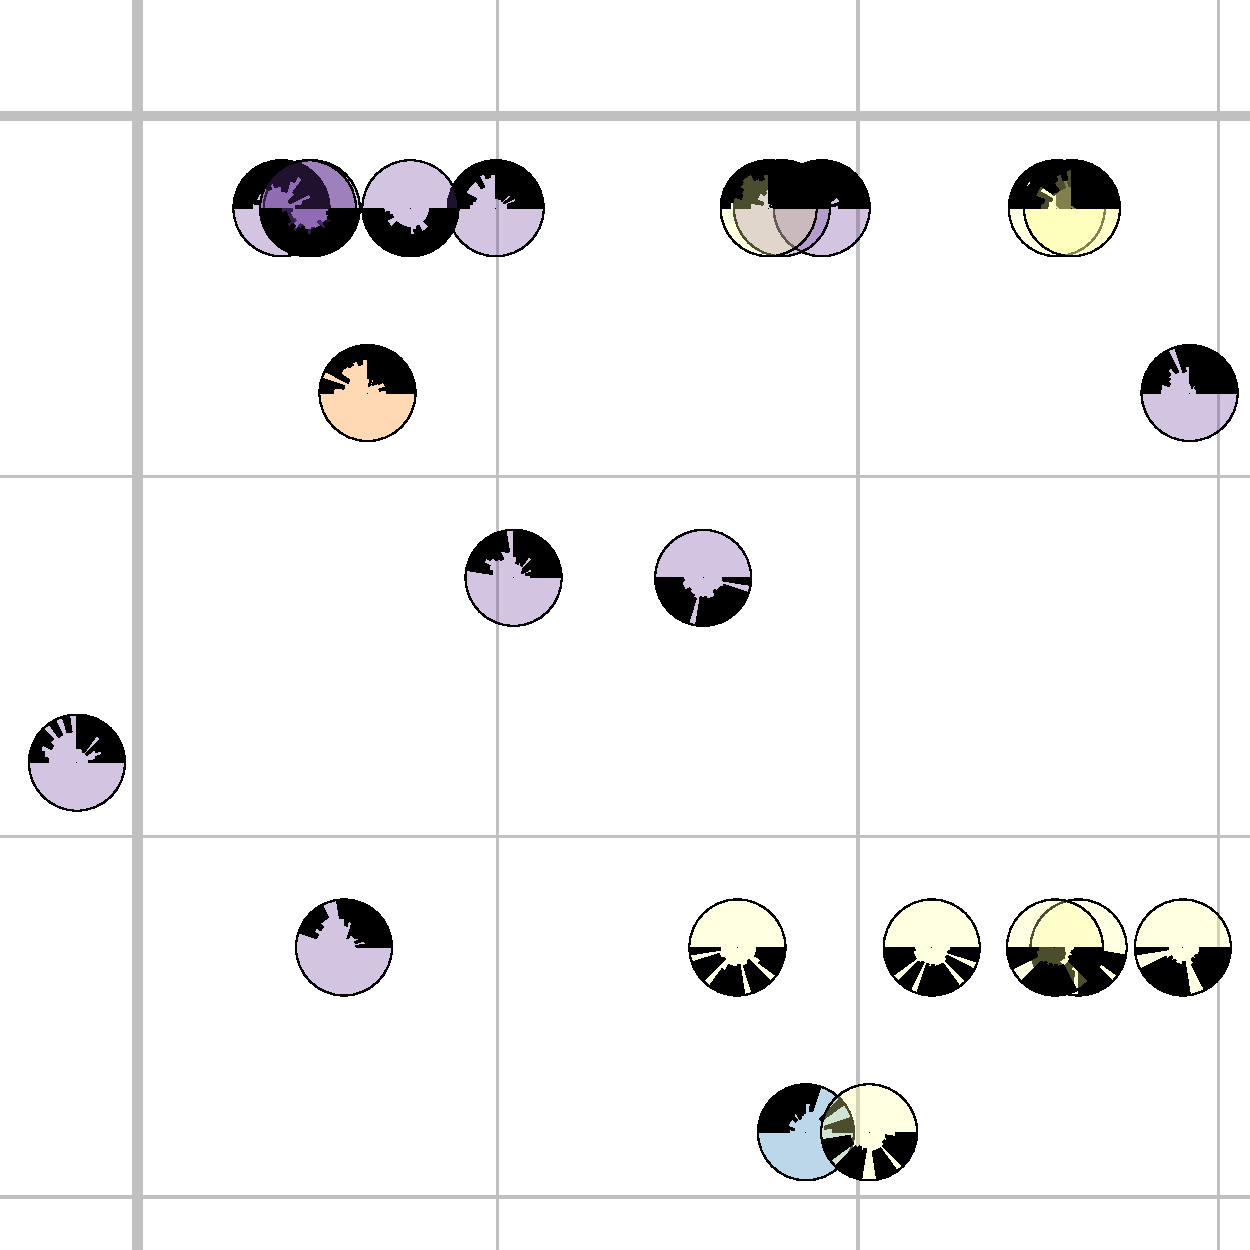
\includegraphics[width=\imgwidth]{infuse/lasso}}};
\end{tikzpicture}%
}
\caption{
The scatterplot view allows users to compare multiple types of rankings.  In the case study, users became curious of the medication features that were chosen by only half of the models.  When reviewing these medications with domain experts, it became clear that features picked by the upper-half algorithms were as clinically significant as those picked by the bottom-half.  This indicates that merging results from feature selection algorithms makes sense for this predictive model.
}
\label{fig:usecase2}
\end{figure*}

\subsection{Insight 1: Data issues}
When the clinical researchers learned of \infuse's capabilities
to compare multiple feature selection algorithms, they decided to
expand their pipeline's feature selection algorithms from 2 to 4.
The team has used Information Gain and Fisher Score extensively
in prior work, and typically uses these same techniques due
to their familiarity and past success.
Nonetheless, the diabetes dataset introduced in Section \ref{sec:running_example} was new to them, and they were unsure which techniques would be the most appropriate. So, they asked their technologists to implement two new techniques: Odds Ratio and Relative Risk.

After all four algorithms were available, they executed their modeling pipeline
using \textit{PARAMO} \cite{paramo} and connected the results to \infuse.
Instantly, the team was surprised at the patterns that the visualization made evident.
The visualization indicated that there seemed to be little agreement between their two
old algorithms, and their two new algorithms for the best features.
The glyphs clearly indicated that many of the features were
highly ranked by two of the four feature selection algorithms,
and unranked by the other two, resulting in glyphs resembling alternating half-circles,
as shown in Figure~\ref{fig:usecase1}.
The team was quick to note that the resulting accuracy across
all four models were not significantly different,
so this non-overlap would have probably gone unnoticed if the
team just looked at resulting predictive scores at the
end of the pipeline as they typically do.

As \infuse gave them the opportunity to
examine multiple algorithms at the feature-level, they were curious as
to why this trend of non-overlapping feature rankings occurred.
They investigated the scores associated with each feature rank
and noticed that many of the features had scores
of $\infty$ from the Relative Risk algorithm.
It turned out there was a bug within the Relative Risk implementation where a
divide by zero error could happen if a feature did not occur
in any of the control patients.  After fixing this bug, they noticed that much of the non-overlap still was evident.  Looking more closely at the algorithms provided a
reason why the two new algorithms behave very differently:  they realized that both of the new algorithms only look at the presence and absence of the feature between the case and controls,
and do not pay attention to the feature values in any other way (e.g. distribution of values).
This is in contrast to the Fisher Score and Information Gain algorithms that take
the actual feature values into account.  This means that for features that are present in both case
and control groups in the same proportion, there is no discrimination value.

One of the team members mentioned, ``Each feature selection algorithm captures different types of information.  \infuse allows you to see what the effect of that information is being captured and gives you insight into the robustness of your predictive model."

As different algorithms will make sense for different purposes depending on the dataset and goals, \infuse provides an ability to inspect the features and determine
which algorithms produce ranked sets of domain-relevant features.

\subsection{Insight 2: Clinically relevant features}
After the data issues were solved, the researchers began investigating
the content of the predictive features.
Using the scatterplot view,
they inspected all of the medications that were ranked by all
feature selection algorithms and folds and found that they
were \textit{antihyperglycemic} medications, which are common treatments to lower the blood sugar of diabetes patients, and made clinical sense to be ranked high.

However, looking towards the center of the scatterplot,
where the features are only ranked by half of the algorithms and folds,
the researchers noticed a cluster of medications that
had half-circle patterns like those described above. This region is highlighted in Figure~\ref{fig:usecase2}. By mouse-hovering these features to read their names, it became clear that those ranked high by the upper-half of the circle (Information Gain and Fisher Score) were as clinically relevant and similar as those ranked by the bottom-half algorithms (Relative Risk and Odds Ratio). This provided feedback that in predictive modeling it is not safe to assume that one single feature selection algorithm is able to detect all possible interesting features and also that having a system like \infuse allows them to build a much richer picture of what kind of feature sets may lead to effective modeling. Without such a tool they would be restricted at evaluating one single algorithm at a time or, at best, restricting the comparison to a small number of features.

%it's not just certain feature selection algorithms that do not a better job overall, but instead might led themselves to finding certain features of various types -- all of which might strengthen the model.

After interacting with the system one of the team members said, ``\textit{If you just use one feature selection algorithm, you're only getting certain types of features. \infuse gives you a guide to what you might be missing. Using a combination type approach [with the Interactive Model Builder] will lead to stronger predictive models.}"

The clinical team is now going to re-think their strategy about how they
build predictive models and may consider using features by merging top
ranked features from different types of feature selection algorithms.
The researchers are convinced that by merging features, in addition
to the interactive model building capability, their predictive models will be improved.

\begin{figure}[ht]
\centering
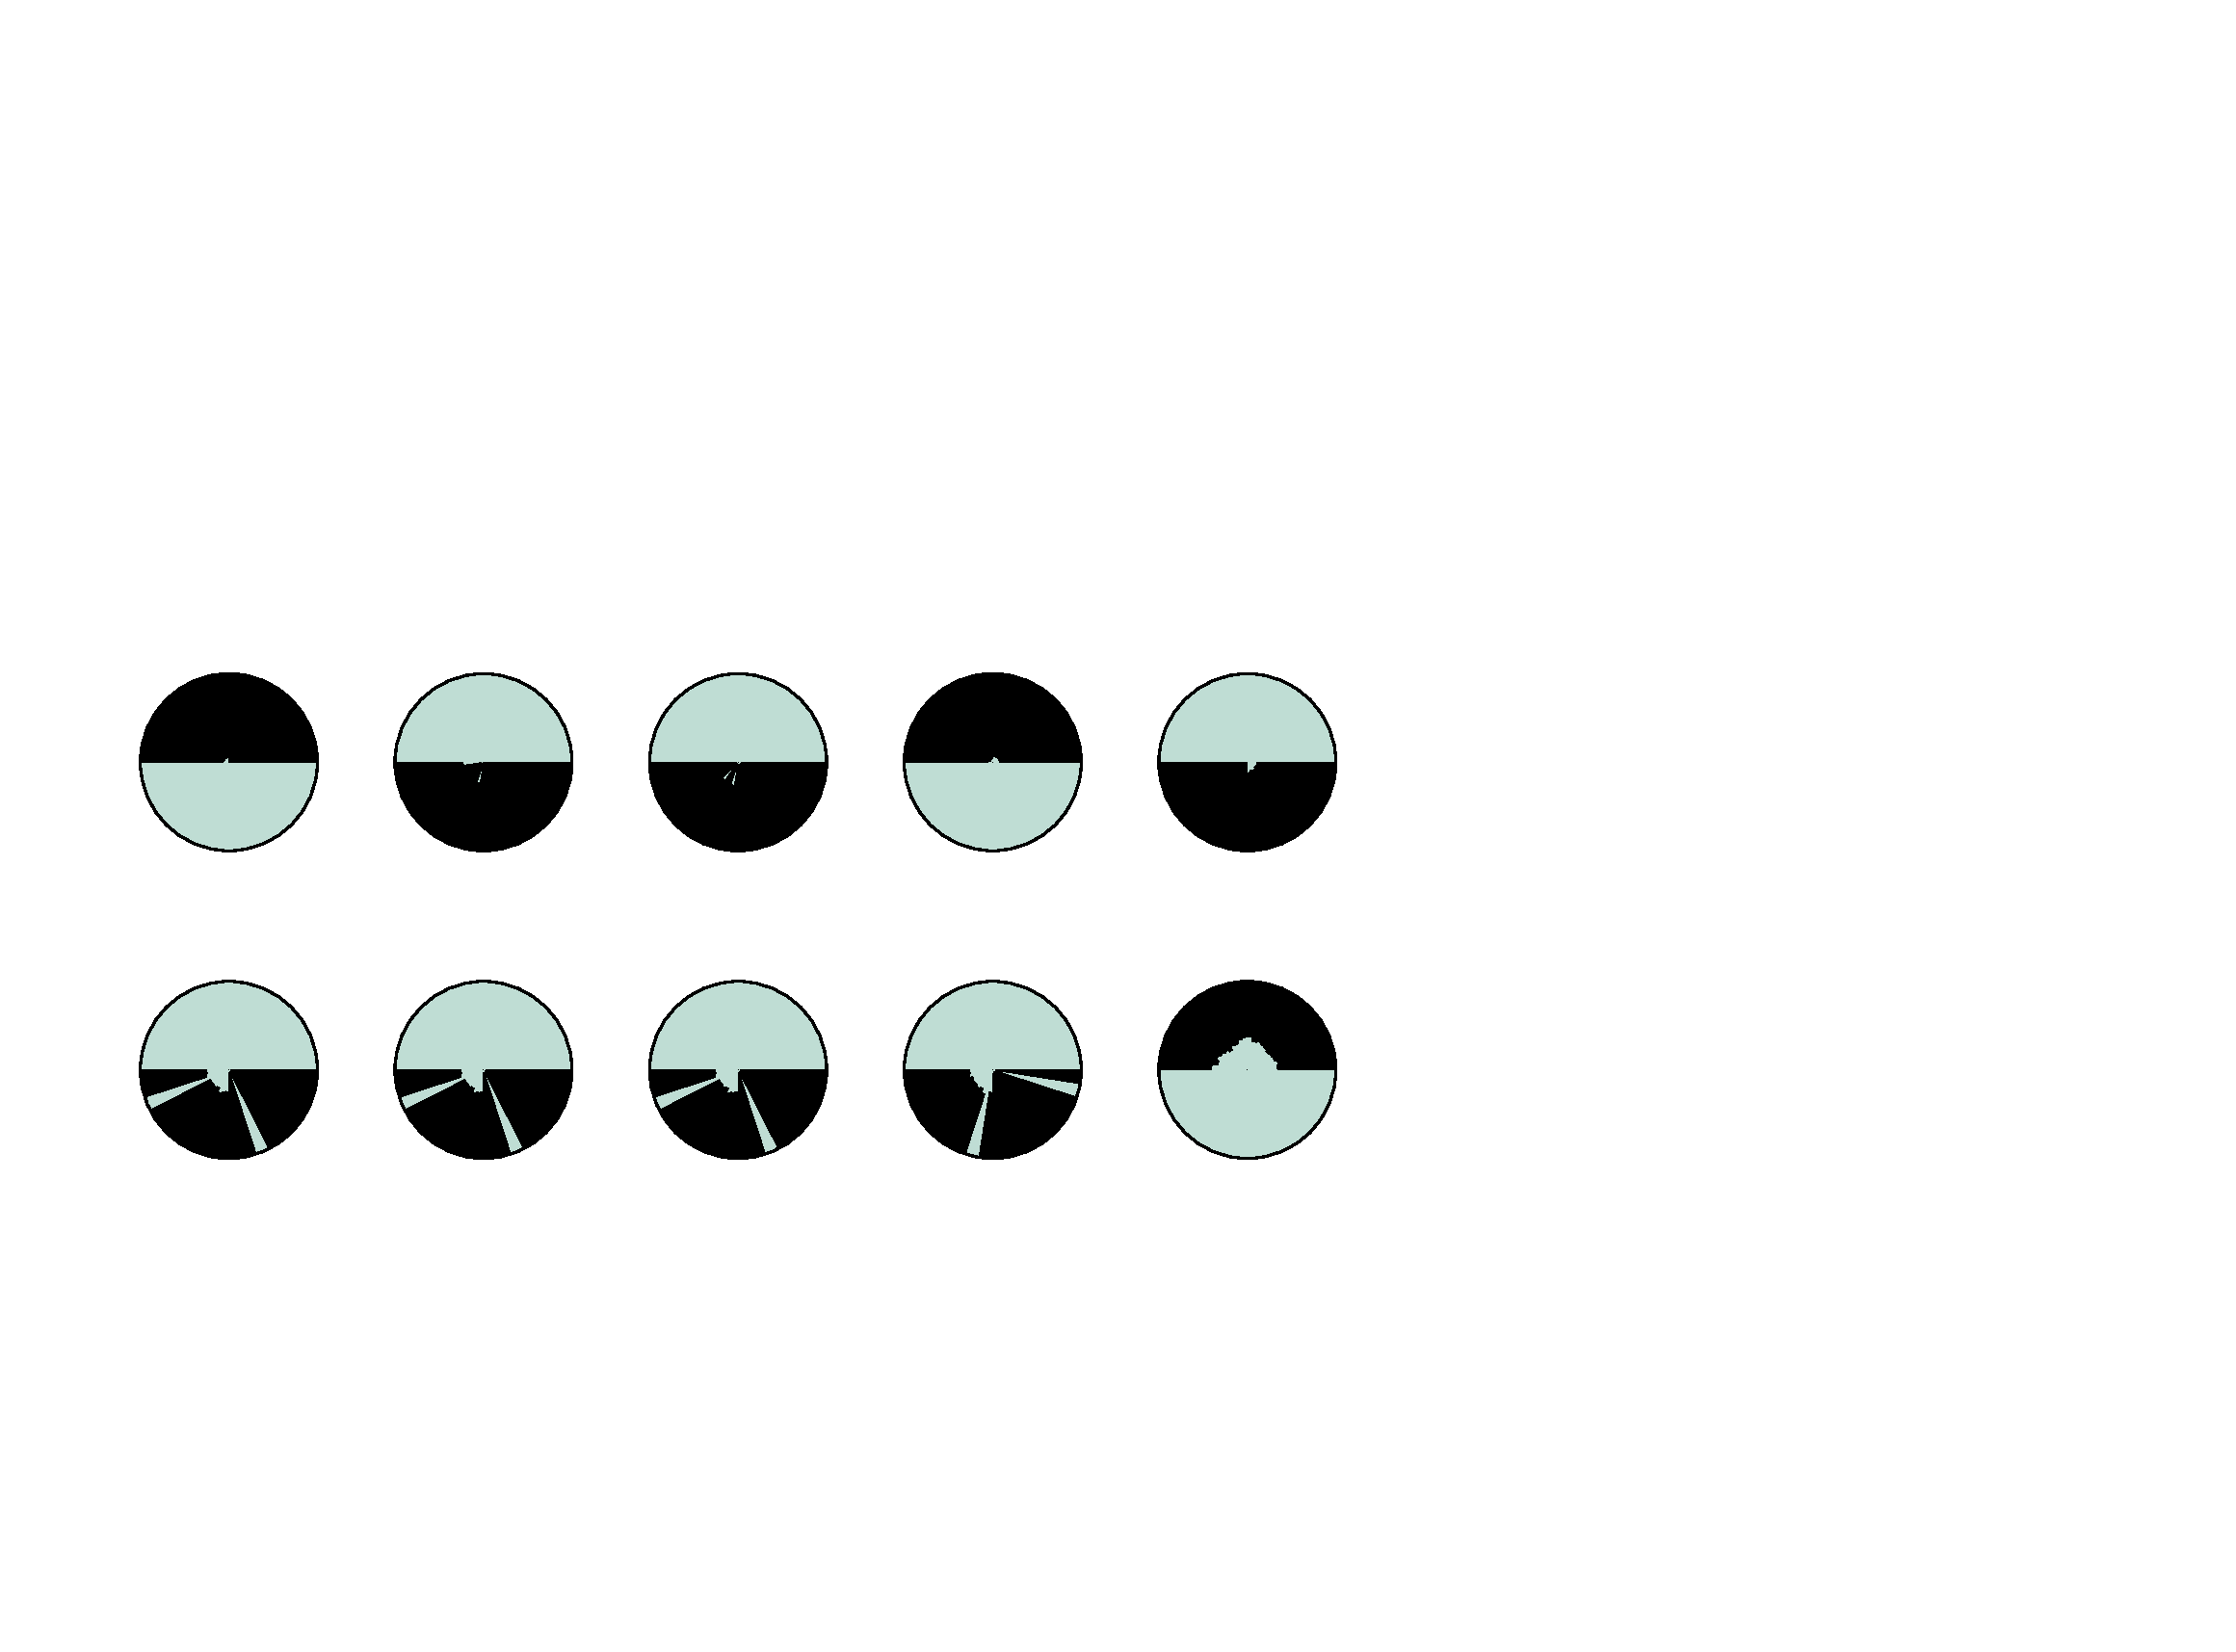
\includegraphics[width=\linewidth]{infuse/usecase1b}
\caption{
The clinical researchers found an interesting pattern among
the glyphs indicating non-overlap of feature selection algorithm results.
These features were highly ranked by 2 of the 4 feature algorithms,
and unranked by the other 2, resulting in glyphs that resemble half-circles.
}
\label{fig:usecase1}
\end{figure}
